\documentclass[a4paper,11pt,BCOR10mm,oneside,headsepline]{scrartcl}
\usepackage{amsmath, mathtools}
\usepackage[ngerman]{babel}
\usepackage[utf8]{inputenc}

\usepackage{typearea, url}
\areaset{17cm}{26cm}
\setlength{\topmargin}{-1cm}
\usepackage{scrpage2}
\pagestyle{scrheadings}

\usepackage[T1]{fontenc}
\usepackage{beramono}
\usepackage{listings}
\usepackage[usenames,dvipsnames]{xcolor}
\usepackage{graphicx}

\ihead{HW1: CIS 631, Parallel Processing}
\ohead{\pagemark}
\chead{}
\cfoot{}

\begin{document}
	
	\begin{center}
		\textbf{\large Homework 1 Report}
	\end{center}\vskip1em
	
	\section{Test Environment}
	I tested my code on department's ix server. It has two sockets with AMD Opteron 6376 on each socket. Each CPU has 8 cores, 16 threads. So, there are 32 hardware threads in total.
	
	\section{Test Results}
		\begin{table}[!htbp]
			\centering
			\begin{tabular}{|c|c|c|c|}
				\hline
				Steps & Accuracy (Pi is 3.1415926535) & Speedup (reduce) & Speedup (atomic add) \\ \hline
				1e6   & \textbf{3.14159}46524                 & 1.30x           & 1.95x                \\ \hline
				1e7   & \textbf{3.141592}8536                 & 5.79x            & 8.93x               \\ \hline
				1e8   & \textbf{3.1415926}736                 & 11.17x           & 15.09x               \\ \hline
				1e9   & \textbf{3.14159265}56                 & 11.99x           & 16.07x               \\ \hline
				1e10  & \textbf{3.14159265}50                & 13.00x           & 16.09x               \\ \hline
			\end{tabular}
			\caption{Integral Method using 32 threads}
		\end{table}
		
		\begin{table}[!htbp]
			\centering
			\begin{tabular}{|c|c|c|}
				\hline
				Steps & Accuracy (Pi is 3.1415926535) & Speedup \\ \hline
				1e7   & \textbf{3.14}11308000               & 16.00x  \\ \hline
				1e8   & \textbf{3.1415}529600               & 18.45x  \\ \hline
				1e9   & \textbf{3.14159}97440               & 23.29x  \\ \hline
			\end{tabular}
		\caption{Monte Carlo Method using 32 threads}
		\end{table}
	
		\begin{figure}[!htbp]
			\centering
			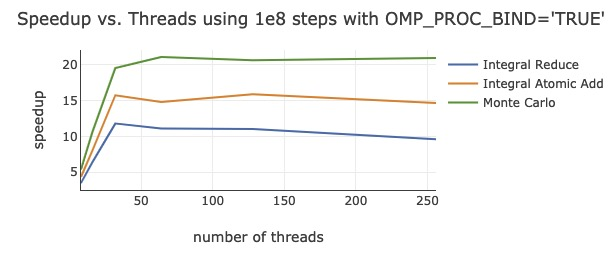
\includegraphics[scale=0.6]{plot}
		\end{figure}

	\section{Findings}
	\begin{itemize}
		\item For both the integral method and Monte Carlo method, we can get better accuracy by increasing the number of steps, but there is a limit on how much accuracy we can get.
		\item Integral method has a better accuracy than Monte Carlo method in general.
		\item We can speedup the computation by increasing number of threads. However, once it passes the number of processors(hardware thread), it may hurt the performance. The figure above shows that we can achieve peak speedup at 32 threads for integral method, and 64 for Monte Carlo method.
	\end{itemize}

\end{document}